\chapter{Fejlesztői dokumentáció}
\label{ch:impl}

Az általam írt céges kódbázis átemelése során szembesültem vele, hogy a függőségeim nagyon mélyre nyúlnak a céges kódbázisban, amit természetesen nem szerettem volna egy az egyben átemelni. A megoldást abban láttam, hogy a függőségekhez saját implementációkat készítek, amik, ha kevésbé komplex módon is de lemodellezik a működést, ami az általam írt kód számára elengedhetetlen a működéshez. A következőkben ezeket a részeket fogom mélyebben bemutatni aztán rátérek a delayed resource lock service bemutatására.

\section{ORM által leképezett adatbázis séma}

Annak ellenére, hogy valódi adatbázis nincs a projekt mögött, azt ORM réteg által leírt adatbázist érdemes bemutatni. A projekt adatbázissémáját a következő ábra illusztrálja.

\begin{figure}[H]
	\centering
	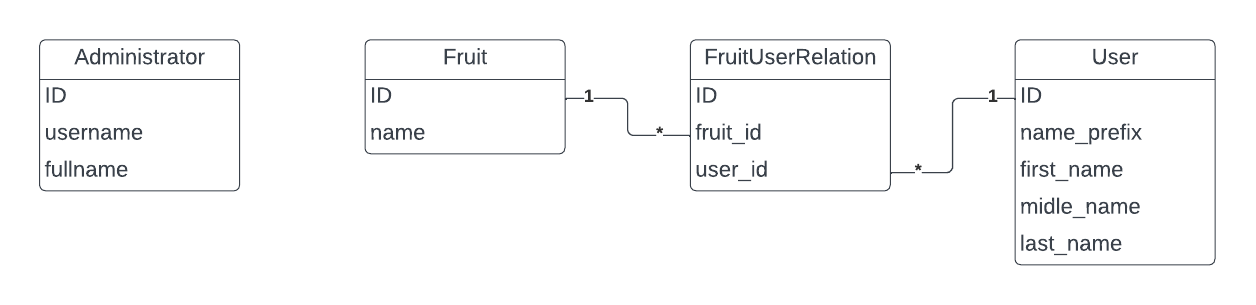
\includegraphics[width=1\textwidth]{images/db_scheme.png}
	\caption{Adatbázis séma diagram}
	\label{fig:main_window}
\end{figure}

\section{Projekt egyszerűsített osztálydiagramja}

A projekt megannyi komponensének a függőségek szemléltetése szempontjából érdemes lehet UML-szerűen ábrázolni, a későbbiekben pedig külön külön lesznek részletezve az egyes komponensek.

\begin{figure}[H]
	\centering
	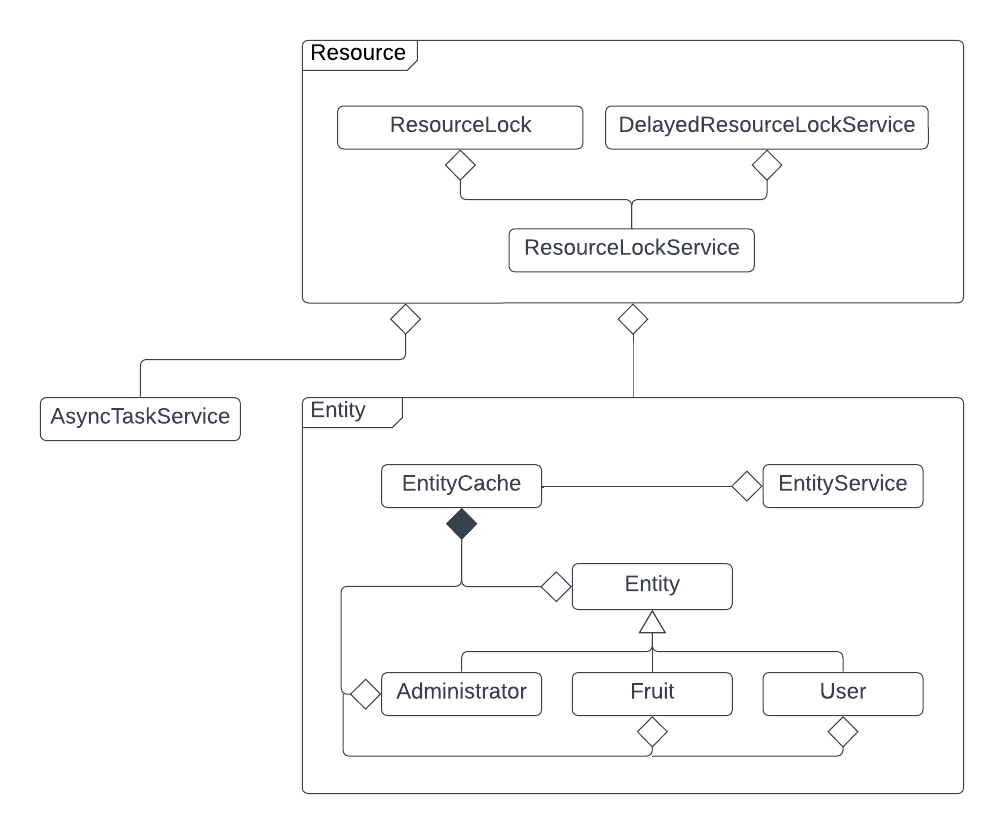
\includegraphics[width=1\textwidth]{images/classdiagram.png}
	\caption{Egyszerűsített osztálydiagram}
	\label{fig:main_window}
\end{figure}

\section{Entitás réteg}

Az entitás réteg szerepe, hogy a programban a nyers SQL írás helyett C++ objektumokkal lehessen típusos módon leírni az adatbázisban végzendő műveleteket. A nyers SQL írás során felmerülő hibák nem derülnek ki csak futásiidőben, emiatt az egyik lényegi tulajdonsága nincs kihasználva a nyelvnek, ami a fordítási időben kiderülő hibák felderítésének lehetősége. Az entitásréteg segítségével a futásidejű hibák átkerülnek a fordítási időbe, ezért a termék nem kerülhet a felhasználók elé olyan állapotban, ami nem felel meg egy stabil elvárható sztenderdnek.

\subsection{Entitások}

Az entitások olyan adatbázisrekordot leképező C++ objektumok, amelyek tartalmazzák az adatbázis rekord mezőit erősen típusos módon privát tagváltozóiban, ehhez pedig publikus getter és szetter van definiálva, hogy kényelmesen lehessen használni. Ezeket nevezzük triviális getternek és triviális szetternek.

Ezek mellett vannak esetenként nem triviális getterek. Erre egy jó példa a felhasználók esetében, a teljes név lekérdezésére létrehozott getter. Ez a tulajdonság egy úgynevezett számított mezője az entitásnak. Ez azt jelenti, hogy adatbázis rekord szinten, illetve entitáson belüli privát adattag szinten sem létezik hozzá mező, viszont másik mezők alapján valamilyen módon megalkotható az adat, aminek a lekérdezése a triviális getterekével azonos szintaktikával történik. Ezekhez a nem triviális getterekhez nem létezik szetter mivel ezeknek nem lenne értelme.

További fontos művelete egy entitásnak, hogy törölhető legyen szükség szerint. Erre a feladatra alkalmas egy paraméter nélküli közvetlenül az entitáson hívható remove művelet, ami eltávolítja azt.

Az entitások fontos része még, hogy rajtuk keresztül lehessen kezelni a hozzájuk kötődő más entitásokkal közös relációikat. Természetesen erre is van lehetőség és az erre kialakított eszközök a reláció típusától függ ezzel is szem előtt tartva a fordítási idejű hibák fontosságát. A relációk esetében megkülönböztetünk 3 fajtát abból a szempontból, hogy egy entitás hány másik entitással állhat kapcsolatban. Ezek lehetnek:

\begin{compactitem}
	\item One to One (Egy az Egyhez)
	\item One to Many (Egy a Többhöz)
	\item Many to Many (Több a Többhöz)
\end{compactitem}

Mivel az entitáson keresztül lehet módosítani azt, hogy mik a vele kapcsolatban lévő entitások és egyszerre csak egy entitással tudunk dolgozni, ezért szintaktikailag elég kétféleképpen különválasztani az eseteinket, a Many to Many sosem fog megjelenni kód szinten.

A One to One esetben az entitások közti reláció is getter és szetter szinten valósul meg szintaktikailag. Ha egy entitáshoz hozzá akarunk rendelni egy másikat csak odaadjuk a szetterének és az a háttérben felépíti a relációt köztük. A getter visszaadja a reláción keresztül az entitást akárcsak egy triviális getter tenné azt egy adattag esetében. Illetve ezek mellett még szükség van az eltávolítás lehetőségére is, ezt akár egy paraméter nélküli remove függvény készítésével is elérhetjük. Ezzel az implementációval le is fedtük ezt az esetet.

A One To Many esetben a szettert felváltja egy add művelet, amivel a már meglévő relációkon túl egy újabbat hozhatunk létre, nem szüntetve meg és nem módosítva a meglévő relációink állapotát. A getterünk ebben az esetben nem pontosan egy darab entitást ad vissza, hanem egy listányit, mivel a több közül nem tudunk válogatni, nincs egy kimondottan jó elem, ezért az alapelv, hogy adjuk vissza az összeset. A relációk megszüntetésére itt két módszert is lehet használni. Az egyik a már korábban megismert remove függvény paraméterezhető verziója, hogy tudja az entitás, hogy a sok közül pontosan melyik entitáshoz kötődő relációját akarjuk lebontani. A Másik Módja ennek a clear függvény lesz, aminek segítségével minden relációt fel tudunk számolni paraméter átadás nélkül. Nézzünk meg erre egy példát publikus inteface kialakítás szintjén.

\lstset{caption={User Entitás header file}, label=src:cpp}
\begin{lstlisting}[language={C++}]
class User
    : public Entity
    , public std::enable_shared_from_this<User>
{
    ...
    
    std::optional<QString> getNamePrefix() const;
    QString getFirstName() const;
    std::optional<QString> getMidleName() const;
    QString getLastName() const;

    // non trivial getters
    QString getFullName() const;

    std::shared_ptr<User> setNamePrefix(const std::optional<QString> &namePrefix);
    std::shared_ptr<User> setFirstName(const QString& firstName);
    std::shared_ptr<User> setMidleName(const std::optional<QString> &midleName);
    std::shared_ptr<User> setLastName(const QString& lastName);

    void remove() override;

    // relations
    const QList<std::shared_ptr<Fruit>> getFruits() const;

    std::shared_ptr<User> clearFruits();
    std::shared_ptr<User> addFruit(std::shared_ptr<db::Fruit> fruitToAdd);
    std::shared_ptr<User> removeFruit(std::shared_ptr<db::Fruit> fruitToRemove);

private:
    std::optional<QString> namePrefix_;
    QString firstName_;
    std::optional<QString> midleName_;
    QString lastName_;

private:
    static int nextId_;
    static constexpr EntityType entityType_ = EntityType::User;
};
\end{lstlisting}

A fentebb lévő kódrészletben jól elkülöníthetőek a korábban említett részek. Az osztálydefiníciót követően a 6. sortól a getterek, a 12. sorban a nem triviális getterek, a 14. sorban a szetterek, a 22. sortól a Many to Many gyümölcsökkel való relációt menedzselő eljárások, végül pedig, bár ez nem a publikus része az osztálynak, a member változóink láthatóak.
A következő komponens bemutatása előtt figyeljük meg, hogy az entitások az Entity ősosztályból származnak le, ahogy az a 2. sorban is látszik. Ennek a ténynek az ismerete később még hasznos lesz. Az ok egyértelműen a futásiidejű polimorfizmus, aminek a segítségével nagy mennyiségű kód duplikáció elkerülésé vált megvalósíthatóvá, illetve az entitások polimorf módon történő tárolása is így került megvalósításra, parametrikus polimorfizmus\footnote{Programozási technika, amely során egy típusparamétertől tesszük függővé egy eljárás vagy egy osztály működését.} vagy type erasure\footnote{Programozási technika, amely során megszabadulunk egy változó típusától, hogy általános módon lehessen kezelni.} helyett.

\subsection{EntityService}

Az entitások amellett, hogy képesek önállóan megannyi művelet elvégzésére, nem tudnak lefedni minden felhasználói esetet teljes mértékben. Az előbbiekben például szembe tűnhetett, hogy a létrehozásukra nem volt egyszerű konstruktor definiálva. Emellett érződik, hogy nem lenne a legbölcsebb csak hagyni ezeket az entitásokat egymástól teljesen függetlenül lebegni, mivel az, hogy ismerjük ezek létezésének tényét valamilyen fejlesztőbarát könnyen kezelhető módon az elengedhetetlen.

Erre a jogosan megfogalmazódó problémára nyújt megoldást az EntityService nevű komponens.

A létrehozásban segítségünkre lesz a create tagfüggvény, ami klasszikus értelemben véve paraméterek nélküli, viszont templateparaméterben átadható neki egy az Entity ősosztályból származó típus, aminek a megkonstruálása az EntityService feladata lesz majd visszaadja a megfelelő altípusú frissen létrehozott entitást. A visszatérési érték típusának is a templateargumentumot használja.

Ezek után, hogy tudunk entitásokat létrehozni a lekérdezésük válik a következő égető hiányossággá amire megoldásul az EntityService szintű gettereket bizonyultak a legkényelmesebb és legjobban használható megoldásnak. Ezek lettek a:

\begin{compactitem}
	\item getById
	\item getAll
	\item getCount
    \item getAllIds
\end{compactitem}

A getterek neve, habár intuitívan utal arra, hogy pontosan mit csinálnak, nézzük meg, hogy mik a helyes viselkedés, amiket velük szembe elvárunk.

A \textbf{getById} pontosan egy paraméteres függvény, ami egy entitás azonosítóját kapja meg paraméterül. Templateargumentumában egy Entitás altípust kap. Elvárt működése a kapott típusnak megfelelő kapott azonosítójú entitás visszaadása.

A \textbf{getAll} paraméter nélküli függvény. Templateargumentumában egy Entitás altípust kap. Elvárt működése a kapott típusnak megfelelő összes entitás visszaadása.

A \textbf{getCount} paraméter nélküli függvény. Templateargumentumában egy Entitás altípust kap. Elvárt működése a kapott típusnak megfelelő entitások számosságának visszaadása.

A \textbf{getAllIds} paraméter nélküli függvény. Templateargumentumában egy Entitás altípust kap. Elvárt működése a kapott típusnak megfelelő összes entitás azonosítójának visszaadása.

Minden különböző entitástípushoz, ami létezik a függvények explicit template specializációval vannak ellátva, hogy a generikus működés jól képeződjön le minden egyes entitás altípusra.

Az osztály a singletinetone\footnote{Az osztályból csak 1 példány hozható létre a program teljes futása alatt.} tervezési minta szerint készült.

Ezeknek az információknak az ismeretében nézzük meg a publikus inteface szintű implementációt:

\lstset{caption={EntityService header file}, label=src:cpp}
\begin{lstlisting}[language={C++}]
class EntityService {
public:
    static std::shared_ptr<EntityService> getInstance();

private:
    EntityService(std::shared_ptr<common::EntityCache> entityCache);

public:
    template<typename Entity_T>
    std::shared_ptr<Entity_T> getById(int id);

    template<typename Entity_T>
    QList<std::shared_ptr<Entity_T>> getAll();

    template<typename Entity_T>
    int getCount();

    template<typename Entity_T>
    QList<int> getAllIds();

    template<typename Entity_T>
    std::shared_ptr<Entity_T> create();

    ...
    
private:
    static std::shared_ptr<EntityService> instance_;

    ...
};
\end{lstlisting}

A fentebb lévő kódrészlet tartalmazza a már írásban taglalt függvénytemplate-ek definícióit, illetve a singletone minta okán privát a konstruktora és publikus statikus genInstance függvénye van ahogy az a 3. és 6. sorban látható.

\subsection{EntityCache}

A fentebbi részekben már kifejtésre került az entitásainkel végezhető műveletek, és az erre létrehozott osztályokat, service-eket. Ebben a részben Az entitásaink tárolásáról tudhatunk meg többet. Mivel a kipróbáló program adatbázis sémával rendelkezik, viszont tényleges adatbázis nincsen a program entitásrétege mögött, valamilyen in memory adatbázisleképezést kellett elkészíteni, hogy ez megfelelően prezentálható legyen, illetve mivel az entitások felépítése alapvetően egy erőforrásigényes folyamat egy gyorsítótár jellegű tároló elkészítése nagyban segíti az alkalmazás reszponzivitását. 

Emellet további és talán legfontosabb szerepe az, hogy az alkalmazásunkban ez a gyorsítótár biztosítja az entitásaink pointerintegritását. Ez azt jelenti, hogy ugyan azt az entitást ha lekérdezzük akkor a cache-ben lévő entitást csak egyezer kell megkonstruálni, onnantól kezdve az egész alkalmazásban ugyan azon az oobjektumot használja minden komponens attól függetlenül, hogy EntityService-en keresztül vagy egy konkrét entitások keresztül kéri le az adott objektumot.

Ebből is látszik, hogy az EntityCache nem közvetlenül használható a felhasználók, fejlesztők számára, hanem az inkább egy az EntityService, és entitás példányok függőségeként létrjövő, őket közvetlenül kiszolgáló segéd objektum. Ennek a célja hogy az Entitások tárolása és konténer objektumokból való visszakeresésének feladata ne az entitásokra háruljon, ezt inkább szervezzük ki egy különálló komponensbe ami dedikáltan csak ezt a feladatot látja el. Nézzük meg az EntityCache-t publikus interface szintjén:

\lstset{caption={EntityCache header file}, label=src:cpp}
\begin{lstlisting}[language={C++}]
class EntityCache {
public:
    static std::shared_ptr<EntityCache> getInstance();

private:
    EntityCache() = default;

public:
    template<typename Entity_T>
    requires std::is_base_of_v<db::Entity, Entity_T>
    const QList<std::shared_ptr<Entity_T>> getCached() {
        ...
    }

    template<typename Entity_T, typename Related_T>
    requires std::is_base_of_v<db::Entity, Entity_T> &&
             std::is_base_of_v<db::Entity, Related_T>
    const QList<std::shared_ptr<Related_T>> getRelatedEntitiesOf(std::shared_ptr<const Entity_T> entity) {
        ...
    }

    template<typename Entity_T>
    requires std::is_base_of_v<db::Entity, Entity_T>
    std::shared_ptr<Entity_T> cache(Entity_T* entityRawPtr) {
        ...
    }

    template<typename Entity_T>
    requires std::is_base_of_v<db::Entity, Entity_T>
    void remove(std::shared_ptr<Entity_T> entity) {
        ...
    }

    template<typename Entity_T, typename Related_T>
    requires std::is_base_of_v<db::Entity, Entity_T> &&
             std::is_base_of_v<db::Entity, Related_T>
    void link(std::shared_ptr<Entity_T> a, std::shared_ptr<Related_T> b) {
        ...
    }

    template<typename Entity_T, typename Related_T>
    requires std::is_base_of_v<db::Entity, Entity_T> &&
             std::is_base_of_v<db::Entity, Related_T>
    void unlink(std::shared_ptr<Entity_T> a, std::shared_ptr<Related_T> b) {
        ...
    }

    template<typename Entity_T, typename Related_T>
    requires std::is_base_of_v<db::Entity, Entity_T> &&
             std::is_base_of_v<db::Entity, Related_T>
    void clearLinksOf(std::shared_ptr<Entity_T> entity) {
        ...
    }

    ...

private:
    static std::shared_ptr<EntityCache> instance_;

private:
    QList<std::shared_ptr<db::Administrator>> admins_;
    QList<std::shared_ptr<db::Fruit>> fruits_;
    QList<std::shared_ptr<db::User>> users_;

    std::set<std::pair<int, int>> fruitUserRelations_;
};
\end{lstlisting}

A fentebbi kódrészletben ismét jól látható módon jelenik meg a singleton tervezési minta. A 3. sorban lévő publikus getInstance felel az objektum lekérdezhetőségéről, és visszaadja az egyetlen objektumra mutató pointert. A 6. sorban lévő privát konstruktor felel az osztály egyetlen példányának megkonstruálásáért. Ez természetesen nem hívható kívülről. Az 58. sorban pedig látható a statikus instance ami az objektumot tárolja.

Ezek után következnek a service lényegi részei. Mivel az osztály minden típusú entitáshoz generikusan kell, hogy működjön egy igen masszív template definíviókkal ellátott osztály törsz fog következni de minden függvény indokoltan használja ezt a nyelvi elemet.

A \textbf{getCached} paraméter nélküli függvény. Templateargumentumában egy Entitás altípust kap. Elvárt működése a kapott típusnak megfelelő összes entitást tartalmazó kollekció érték szerinti visszaadása.

A \textbf{getRelatedEntitiesOf} egy paraméterrel rendelkező függvény, ami egy entitás példányt kap. Templateargumentumában kettő Entitás altípust kap, az első megegyezik a paraméterének típusával, a másik egy a paraméterrel relációba állítható Entity altípus. Elvárt működése a kapott entitással relációban lévő összes entitás visszaadása.

A \textbf{cache} egy paraméterrel rendelkező függvény ami egy entitás példányt kap viszont raw pointer-en keresztül. Templateargumentumában egy Entitás altípust kap, ez megegyezik a paraméterének típusával. Elvárt működése a kapott entitás raw pointer teljes értékű entitássá alakítása, és ownership kialakítása. Ezt követően pedig az entitás visszaadása.

A \textbf{remove} egy paraméterrel rendelkező függvény, ami egy entitás példányt kap. Templateargumentumában egy Entitás altípust kap, ez megegyezik a paraméterének típusával. Elvárt működése a kapott entitás kitörlése az azt tartalmazó kollekcióból, és annak destruálása.

A \textbf{link} kettő paraméterrel rendelkező függvény, ami két entitás pédányt kap. Templateargumentumában két Entitás altípust kap, ez megegyezik a paraméterének tapott entitások típusával. Elvárt működése a kapott entitások közötti reláció kialakítása.

A \textbf{unlink} kettő paraméterrel rendelkező függvény, ami két entitás pédányt kap. Templateargumentumában két Entitás altípust kap, ezek megegyeznek a paraméterének kapott entitások típusával. Elvárt működése a kapott entitások közötti reláció megszüntetése.

A \textbf{clearLinksOf} egy paraméterrel rendelkező függvény ami egy entitás pédányt kap. Templateargumentumában két Entitás altípust kap, az első megegyezik a paraméterének kapott entitások típusával, a másik szintén egy Entitás altípus. Elvárt működése a kapott entitás összes relációjának megszüntetése a templétargumentumként kapott másik entitástípus összes példányával.

A forráskód privát szekciójában, a 61. sortól kezdve, láthatóak az entitásokat tartalmazó kollekciók, illetve, a 65. sortól, az egyes entitás típusok közötti relációkat tartalmazó konténerek.

\subsection{Az entitásréteg interakcióji a komponensek között}

A következő részekben nézzünk meg néhány érdekes interakciót a korábban megismert Entitás réteg komponensei között. Először vessünk egy pillantást az Entitások létrehozásának folyamatára.

\lstset{caption={Alma nevű gyümölcs entitás létrehozása}, label=src:cpp}
\begin{lstlisting}[language={C++}]
auto aple = entityService->create<db::Fruit>()
                ->setName("Alma");
\end{lstlisting}

A fentebbi mintakódban az látható, ahogy az EntityService segítségével létrehozunk egy Gyümölcs entitást, majd ennek az entitásnak beállítjuk a név tulajdonságát a az Alma szöveges literálra, és végül az egész kifejezés kiértékelése után a visszatérési értéket berakjuk egy aple nevű változóba. Nézzük meg, hogy az egyes részek miként működnek és pontosan merre jár a vezérlés ennek az igen kényelmesen használható, intuitív kódrészlet kiértékelése közben.
Az első kiértékelésre kerülő kifejezés az entityService objektum példányon meghívott create utasítás lesz.

\lstset{caption={Create belső működése}, label=src:cpp}
\begin{lstlisting}[language={C++}]
template<>
std::shared_ptr<db::Fruit> common::EntityService::create() {
    return entityCache_->cache(new db::Fruit());
}
\end{lstlisting}

A vezérlés az EntityService, Fruit típussal történő explicit templatespecializációjába fog megérkezni, ahol az entityCache objektum példányán meghívjuk a cache függvényt. Ez paraméterül kap egy helyben default konstruktorral, a heap-en létrehozott gyümölcs típusú entitást.

\lstset{caption={Fruit belső működése}, label=src:cpp}
\begin{lstlisting}[language={C++}]
Fruit::Fruit()
    : Entity(nextId_++)
{}
\end{lstlisting}

Itt a konstruktor létrehozza az entitást, és meghívja az ősének az Entity-nek a konstruktorát, aminek továbbadja a nextId\_ nevű statikus változót, rögtön ez követően meg is növelve azt. Ennek segítségével érhető el az entitások Id-jának inkrementális növelése. Ezt követi az Entity konstruktora.

\lstset{caption={Entity belső működése}, label=src:cpp}
\begin{lstlisting}[language={C++}]
Entity::Entity(int id)
    : entityCache_(common::EntityCache::getInstance())
    , id_(id)
{}
\end{lstlisting}

Itt az entitásban lévő EntityCache példány megkapja az EntityCache::getInstance függvénye által visszaadott egyetlen objektumra mutató pointert. Emellett elvégzi a másik nagyon fontos feladatát, ami az Id beállítása. Ezt természetesen a member initializer list-je segítségével teszi meg, mivel az a best practice, másrészt pedig mivel a változó const megszorítása miatt nem lehetne ezt a konstruktor törzsében megtenni.

Ezt követően a vezérlés visszatér az EntityService-be, ahol végül pedig a kifejezés visszatérési értékével tér vissza ő maga is, de ez előtt a vezérlés tovább halad az EntityCache cache nevű függvényre a frissen megkonstruált pointert átadva annak.

\lstset{caption={cache belső működése}, label=src:cpp}
\begin{lstlisting}[language={C++}]
template<typename Entity_T>
requires std::is_base_of_v<db::Entity, Entity_T>
std::shared_ptr<Entity_T> cache(Entity_T* entityRawPtr) {
    auto entity = std::shared_ptr<Entity_T>(entityRawPtr);
    getListOfType<Entity_T>().append(entity);
    return entity;
}
\end{lstlisting}

Itt pedig megtörténik a már korábban megismert függvény feladatának beteljesítése, ami az entitás feletti ownership kialakítása, és eltárolása. Ez technikailag egy std::shared\_ptr használatával teszi meg. Az erről készített másolat bekerül a belső kollekcióban ami a templateargumentum alapján kerül kiválasztásra a getListOfType privát függvény segítségével. Ezt követően a függvény visszatér az eredeti pointer-rel és bezárul a kör.

A vezérlésünk visszatér a vermünk felszínére ahol a következő utasítás a már megkonstruált entitás nevének beállítása. Ez itt Már természetesen a Fruit entitás egyik szettere lesz.

\lstset{caption={Fruit belső működése}, label=src:cpp}
\begin{lstlisting}[language={C++}]
std::shared_ptr<db::Fruit> Fruit::setName(const QString& name) {
    name_ = name;
    
    return shared_from_this();
}
\end{lstlisting}

Itt egy triviális settert láthatunk egy Builder tervezési mintával ellátva amiben annyi plusz csavar van, hogy a builder a this-t referencia helyett egy std::shared\_ptr-be csomagolva adja vissza. Ennek köszönhető, hogy a hívó fél a szetter használata után is értékül adhatja egy változónak az entitását.

Ezt ki is használva a teljes kifejezés visszatérési értékét odaadjuk a változónak és ezzel létre is jött az Alma nevű Gyümölcs típusú entitás.

\section{Delayed resource lock service}

A fentebb leírt eszközök működése mellett felmerülhetnek további olyan problémák, amikre ez az eszköztár nem nyújt teljes körű megoldást. Az egyik ilyen Felhasználói eset például, ha egy folyamatot meg akarunk várakoztatni az erőforrások elérhetetlensége miatt akkor erre nemigazán van jó módszer, illetve az erőforrásoknak nem tájékozódunk a felszabadulásáról ezért az, hogy mennyi időt kell várni azt valamilyen módon a felhasználónak kell kitalálnia. A DelayedResourceLockService ennek a kimondott esetnek a kezelésére lett megalkotva. 

Abban az esetben, ha a folyamat jellege miatt nem érdekes, hogy mikor lesz elvégezve csak az a célunk, hogy előbb utóbb a végrehajtás történjen meg A DelayedResourceLockService lesz a jó választás. A service egy teljesen a felhasználótól függő névtelen függvényt kap paraméterül, és egy halmaznyi lefoglalandó erőforrást, ami a folyamat elvégzéséhez szükségesek. A működése egyszerű, igazából kettő fő esetre lehet szétválasztani.

Az első eset az amikor a folyamat által igényelt paraméterül átadott erőforrások elérhetőek. Ekkor ezek gond nélkül lefoglalásra kerülnek, a zár birtokbavétele megtörténik. Ezt követően A folyamat lezajlik, ennek végeztével az erőforrások felszabadulnak. Ez az eset ekvivalens a ResourceLockService azon esetével amikor az erőforrások lefoglalása megtörténik. Ez egyébként a tervezés során elvárt viselkedés is volt.

A másik eset amikor a szükséges resourcok lefoglalása valamilyen hibára fut, természetesen ez csak azt jelenti, hogy más éppen dolgozik azokkal. Ekkor a felhasználótól paraméterben kapott névtelen függvény az erőforrásokkal együtt bekerül egy várakoztatási sorba. Új szál nem indul ezekkel egyidejűleg, hogy ez ne csökkentse a thread pool-ban lévő használható szálak mennyiségét. Ebből a várakoztatási sorból az elemek 2 féleképpen kerülhetnek ki.

Az egyik módja, ha a ResourceLockService elemmitál egy szignált, ez jelzést ad arról, hogy az eddigi lefoglalt resourcok halmaza megváltozott. Erre a jelzésre figyelve a DelayedResourceLockService végig iterál a várakoztatási soron, és megkísérli az újonnan felszabadult erőforrásoknak megfelelő elemeket lefuttatni. Amennyiben ez sikeresen lezajlik, a folyamat lezajlott az elem kikerül a várakoztatási sorból. A bennmaradó elemeken ismét végig iterálunk a jelzések érkezésével, így fokozatosan elfogyasztva a lista teljes tartalmát.

A másik módja az elemek listából való eltávolításának az, ha az elem által igényelt erőforrások nem szabadulnak fel az elemnek megadott időtúllépési limit tartalma alatt. Az elemeknek meghatározható a felhasználó által egy maximális időkorlát amíg bennmaradhat egy elem a várakoztatási sorban. Amint a várakoztatási sorban töltött idő átlépi a maximálisan dedikált időt a feladat elvégzésére, a feladat az időtúllépési státuszba lép. Ekkor a feladat végrehajtása nem valósul meg, A várakoztatási sorból kikerül a végrehajtás nélkül.

Tipikus példája ez a kiéheztetésnek és ez a mechanizmus az örökké várakozó folyamatok beragadását hivatott elkerülni. De mit tudunk tenni abban az esetben, ha a folyamatunkat kiéheztették? Erre a kérdésre is a komponens felhasználója kell, hogy fel legyen készülve hisz a komponens csak a folyamatok megvárakoztatásáért és végrehajtásáért felel. Ha egy folyamat kiéheztetése megtörténik akkor az a hatáskörén kívül eső probléma, ami ennél jóval mélyebben is gyökerezhet. A felhasználó erre gondolva adhat egy opcionális paraméterként egy időtúllépés esetén lefuttatandó folyamatot. Ebben megkísérelhet tenni a kiéheztetést végző folyamatok ellen vagy logot helyezhet el a hibajelenség detektálhatóságának érdekében és későbbi javíthatóságának megkönnyítéséért. Az a program, ami kiéhezteti a saját folyamatait eleve rosszul működik tehát ez a rész igazából egy megoldás a végső esetre, de jobb, hogyha van és sosincs kihasználva, mintha nem lenne és egyszer egy ilyen jellegű hiba felmerülése során egy jóval nagyobb kódbázist kell kielemezni a hiba helyének feltárása érdekében.

Nézzük meg az osztályt kicsit technikaibb szemmel, hogy a működések hátterében levő mechanizmusokról kiderüljenek a részletek.

\subsection{Függőségek}

A komponens explicit függőségei az AsyncTaskService az aszinkron folyamatok kezelésére hivatott komponens, és a ResourceLockService ami segítségével az erőforrások lefoglalását végzi a komponens. Ezeket konstruktorparaméterben kapja.

\subsection{Belső típusok}

A komponens egy privát belső típussal rendelkezik, név szerint az AsyncLock-kal. Ebben a típusban tudjuk eltárolni a várakozó folyamatokat.

\lstset{caption={AsyncLock belső típus}, label=src:cpp}
\begin{lstlisting}[language={C++}]
struct AsyncLock {
    std::variant<common::CallerContext, QString> contextOrTag_;
    std::map<common::LockableResource, common::ResourceLockType> resources_;
    AsyncTaskPtr task_;
    std::unique_ptr<QObject> guard_ = std::make_unique<QObject>();

    ...
};
\end{lstlisting}

Itt látható a felhasználó által megadott task, az erőforrások map-je, és egy guard objektum, ami egy nyers QObject. Erre a timeout task miatt van szükség.

\subsection{Tagváltozók}

A tagváltozóink között az osztályunk két függősége mellett egy lista látható, ami AsyncLock belső típussal rendelkező elemeket tárol. Ez a technikai implementációja a várakoztatási sornak. Közvetlenül alatta látható egy std::mutex aminek a szerepe a lista szinkronizációja. A lista akár egyszerre több szálból is módosulhat. A lehetséges racecondition-ök elkerülése végett a lista minden művelete lelokkolja a mutexet az implementációban. Alatta található két std::atomic-ba wrapp-elt logikai érték, ezek szerepe a lista feldolgozása során van.

\lstset{caption={Tagváltozók}, label=src:cpp}
\begin{lstlisting}[language={C++}]
std::shared_ptr<common::IResourceLockService> resourceLockService_;
std::shared_ptr<common::AsyncTaskService> asyncTaskService_;

QList<std::shared_ptr<AsyncLock>> asyncLocks_;
std::mutex asyncLocksMutex_;

std::atomic_bool inProgress_      = false;
std::atomic_bool hasMissedSignal_ = false;
\end{lstlisting}

\subsection{Publikus interface}

A publikus interface-en található kettő függvény, ami az adminisztrátor és rendszer szintű folyamat futtatásra lett megalkotva. A paraméterlistájuk nagyrész megegyezik így ezt egyben fogom kifejteni.

Az első paraméter az adminisztrátor szintű hívás esetén egy CalleContext kontextust tartalmazó objektum, ami az adminisztrátor beazonosításában játszik szerepet. A rendszer esetben ez egy egyszerű szöveges változó, ami a rendszer beazonosításában játszik szerepet.

A második paraméter a már korábban megismert LockableResource kulcsokhoz ResourceLockType kulcsaikat rendelő map, ez itt is a lefoglalandó erőforrásokat és azok írási vagy olvasási típusú zárolásának többletadatát hordozza.

A harmadik paraméter a természetesen a task aminek az elvégzéséhez a második paraméterben átadott erőforrások szükségesek. 

A negyedik paraméter egy időtúllépési korlát, amit milliszekundumban adhatunk meg. Ezzel megszabhatjuk, hogy a Folyamat által igényelt, második paraméterként átadott erőforrások, rendelkezésre nem állásának állapota maximálisan mennyi ideig fogadható el a feladat elvégzésének szempontjából. Fontos, hogy ez az időtúllépés csak a várakozásra vonatkozik, ha a folyamat már elkezdődött akkor, a futásának ideje nem számít bele az időtúllépésnek megszabott felső határba, tartson bármilyen sokáig.

Ezt követően következik az utolsó paraméter, ami egyben az első opcionális paraméter, az időtúllépési task. Ez akkor fut le, ha a kijelölt milliszekundumnyi idő alatt nem sikerül az erőforrások lefoglalása.

\lstset{caption={Publikus interface}, label=src:cpp}
\begin{lstlisting}[language={C++}]
void addAsyncLock(CallerContext context,
                  std::map<LockableResource, ResourceLockType> resources,
                  AsyncTaskPtr task,
                  int timeoutMs,
                  AsyncTaskPtr timeoutTask = nullptr) override;

void addAsyncSystemLock(QString tag,
                        std::map<LockableResource, ResourceLockType> resources,
                        AsyncTaskPtr task,
                        int timeoutMs,
                        AsyncTaskPtr timeoutTask = nullptr) override;
\end{lstlisting}

\section{Tesztelési tervezet}

A tesztelés során a DelayedResourceLockService és az AsyncTaskService integrációs tesztjei kerültek megvalósításra. Ennek oka az, hogy az AsyncTaskService szorosan összefügg a működéssel az aszinkron mivoltából kifolyólag és nem lehetne jól mock-olni a működését. A másik függőség, ami a ResourceLockService természetesen jól mock-olható objektum, így az ilyen módon szerepel a tesztelésben. A tesztek során a DelayedResourceLockService teljeskörű tesztje valósul meg törekedve a minél nagyobb kódbázis lefedettségének elérésére és a minél változatosabb végrehajtásokra.

\begin{center}
	\begin{longtable}{ | p{0.25\textwidth} | p{0.7\textwidth} | }
		
		\hline
		\multicolumn{2}{|c|}{\textbf{Integrációs tesztek}}
		\\ \hline
		
		\emph{Teszteset} & \emph{Leírás}
		\\ \hline \hline
		\endfirsthead % első oldal fejléce
		
		\hline
		\emph{Teszteset} & \emph{Leírás}
		\\ \hline \hline
		\endhead % többi oldal fejléce
		
		\hline
		\endfoot % többi oldal lábléce
		
		\endlastfoot % utolsó oldal lábléce
		
        \emph{single AsyncLock AvailableResources} &
        A teszt azt vizsgálja, hogy elérhető erőforrások mellett egy egyedüliként indított adminisztrátor jogosultságú folyamat lefut-e.
		\\ \hline
		
		\emph{single AsyncSystemLock AvailableResources} &
		A teszt azt vizsgálja, hogy elérhető erőforrások mellett egy egyedüliként indított rendszer jogosultságú folyamat lefut-e.
		\\ \hline
		
		\emph{multiple AsyncLock AvailableResources} &
		A teszt azt vizsgálja, hogy elérhető erőforrások mellett több egyidejűleg indított adminisztrátor jogosultságú folyamat lefut-e.
		\\ \hline
		
		\emph{multiple AsyncSystemLock AvailableResources} &
		A teszt azt vizsgálja, hogy elérhető erőforrások mellett több egyidejűleg indított rendszer jogosultságú folyamat lefut-e.
		\\ \hline
		
		\emph{single AsyncLock LockedResources} &
		A teszt azt vizsgálja, hogy lefoglalt erőforrások mellett egy egyedüliként indított adminisztrátor jogosultságú folyamat bekerül-e a várakoztatási sorba, majd a megadott idő elteltével kikerül-e belőle az időtúllépés miatt.
		\\ \hline
		
		\emph{single AsyncSystemLock LockedResources} &
		A teszt azt vizsgálja, hogy lefoglalt erőforrások mellett egy egyedüliként indított rendszer jogosultságú folyamat bekerül-e a várakoztatási sorba, majd a megadott idő elteltével kikerül-e belőle az időtúllépés miatt.
		\\ \hline
		
		\emph{single AsyncLock LockedResources WitchThenFreesUp} &
		A teszt azt vizsgálja, hogy lefoglalt erőforrások mellett egy egyedüliként indított adminisztrátor jogosultságú folyamat bekerül-e a várakoztatási sorba, majd később amikor a megfelelő erőforrások felszabadulnak, a sorban lévő folyamat elindul-e és végrehajtja-e a neki kijelölt feladatot. Illetve, hogy ennek végeztével kikerül-e a sorból.
		\\ \hline
		
		\emph{single AsyncSystemLock LockedResources WitchThenFreesUp} &
		A teszt azt vizsgálja, hogy lefoglalt erőforrások mellett egy egyedüliként indított rendszer jogosultságú folyamat bekerül-e a várakoztatási sorba, majd később amikor a megfelelő erőforrások felszabadulnak, a sorban lévő folyamat elindul-e és végrehajtja-e a neki kijelölt feladatot. Illetve, hogy ennek végeztével kikerül-e a sorból.
		\\ \hline

		\emph{two Concurrent AsyncLock} &
		A teszt azt vizsgálja, hogy két egymással az erőforrásokon konkuráló adminisztrátor jogosultságú folyamat gond nélkül le tud-e futni. A sorrendjük természetesen nem determinisztikus tehát a teszt a futásuk sorrendjéről nem feltételez semmit.
		\\ \hline

  	\emph{two Concurrent AsyncSystemLock} &
		A teszt azt vizsgálja, hogy két egymással az erőforrásokon konkuráló rendszer jogosultságú folyamat gond nélkül le tud-e futni. A sorrendjük természetesen nem determinisztikus tehát a teszt a futásuk sorrendjéről nem feltételez semmit.
		\\ \hline
  
		\caption{Automatizált integrációs tesztek összegzése}
		\label{tab:example-3}		
	\end{longtable}
\end{center}